\section*{The dataset features}

\subsection*{The RMM matrix}
Most of the features in the analysis are elements in the so called Rapidity-Mass (RMM) matrix inspired by the work of Chekanov \cite{Chekanov_2019}.
\par
!! Motivation for using such a matrix in machine learning $\to$ hint to highly uncorrolated feats!!
\par
Its composition is determined as a square matrix of $1 + \sum_{i=1}^{T}N_i$ columns and rows, where T is the total number of objects (i.e jets, electrons etc.),
and $N_i$ is the multiplicity of a given object. In the case of the same number of a given object for all objects, we can denote the RMM matrix as a 
TmNn matrix, where m is the multiplicity of T, and n is the number of particle per type. Thus there is already room for evaluation, as the combination of number of objects 
and the number of each object type highly affects the analysis as well as computational resources. Each cell in the matrix contains information about
either single og two particle properties. An example is shown in matrix \ref{eq:rmmmatrix}.

\begin{equation}\label{eq:rmmmatrix}
\begin{pmatrix}
    \boldsymbol{e}_{T}^{miss} & m_T(j_1) & m_T(j_2) &  m_T(e_1) &  m_T(e_2)\\
    h_L(j_1) & \boldsymbol{e_T}(j_1) & m(j_1, j_2) & m(j_1, e_1) & m(j_1, e_2)\\
    h_L(j_2) & h(j_2, j_1) & \delta \boldsymbol{e_T}(j_2)& m(j_2, e_1) & m(j_2, e_2)\\
    h_L(e_1) & h(e_1, j_1) & h(e_1, j_2) & \boldsymbol{e_T}(e_1) & m(e_1, e_2)\\
    h_L(e_2) & h(e_2, j_1) & h(e_2, j_2) & h(e_2, e_1) & \delta \boldsymbol{e_T}(j_2)\\
\end{pmatrix}
\end{equation}

In matrix \ref{eq:rmmmatrix} we have the RMM matrix for a T2N2 system, in other words we have two types of particles, jets and electrons, where each type has
two particles. The matrix itself is partitioned into three parts. The diagonal represents energy properties, the upper triangular represents mass properties, 
and the lower triangular represents longitudal properties related to rapidity. The diagonal has three different properties, $\boldsymbol{e_T^{miss}}$, $\boldsymbol{e_T}$ and $\delta\boldsymbol{e_T}$. 
$\boldsymbol{e_T^{miss}}$ is placed in the $(0,0)$ in the matrix. It accounts for the missing energy for the system, which is of high interest for this analysis due to
the search for heavy neutrinos. $\boldsymbol{e_T}$ is the transverse energy defined as 
\begin{equation*}
    \boldsymbol{e_T} = \sqrt{m^2 + p_T^2}
\end{equation*}
but for light particles such as electrons, this can be approximated to $\boldsymbol{e_T} \approx p_T$. $\delta\boldsymbol{e_T}$ is the transverse energy imbalance.
It is defined as 
\begin{equation*}
    \delta\boldsymbol{e_T} = \frac{E_T(i_n-1) - E_T(i_n)}{E_T(i_n-1) + E_T(i_n)}, \, n = 2, ..., N.
\end{equation*}
The first columm in the RMM matrix, with the exeption of the first element, is related to the longitudal property of the given particle. 
It is defined as
\begin{equation*}
    h_L(i_n) = C(\cosh{(y)} - 1),
\end{equation*}
where C is a constant to ensure that the average $h_L(i_n)$ values do not deviate too much from the ranges of the invariant masses of the transverse masses, found to be $0.15$\cite{Chekanov_2019}. 
y is the rapidity of the particle, and $i_n$ is the particle number. On the lower triangle we have the longitudal properties of the combinations of particles. Similar to $h_L(i_n)$,
this property is defined as 
\begin{equation*}
    h(i_n, j_k) = C(\cosh{(\Delta y)} - 1),
\end{equation*}
where $\Delta y = y_{i_n} - y_{j_k}$ is the rapidity difference for particle $i_n$ and $j_k$. 

\subsection*{Implementation of the RMM matrix}
An example of the RMM matrices used in this thesis is shown in figure \ref{fig:rmm_singular_events} below:


\begin{figure}[h!]
    \centering
    \begin{subfigure}{.7\textwidth}
        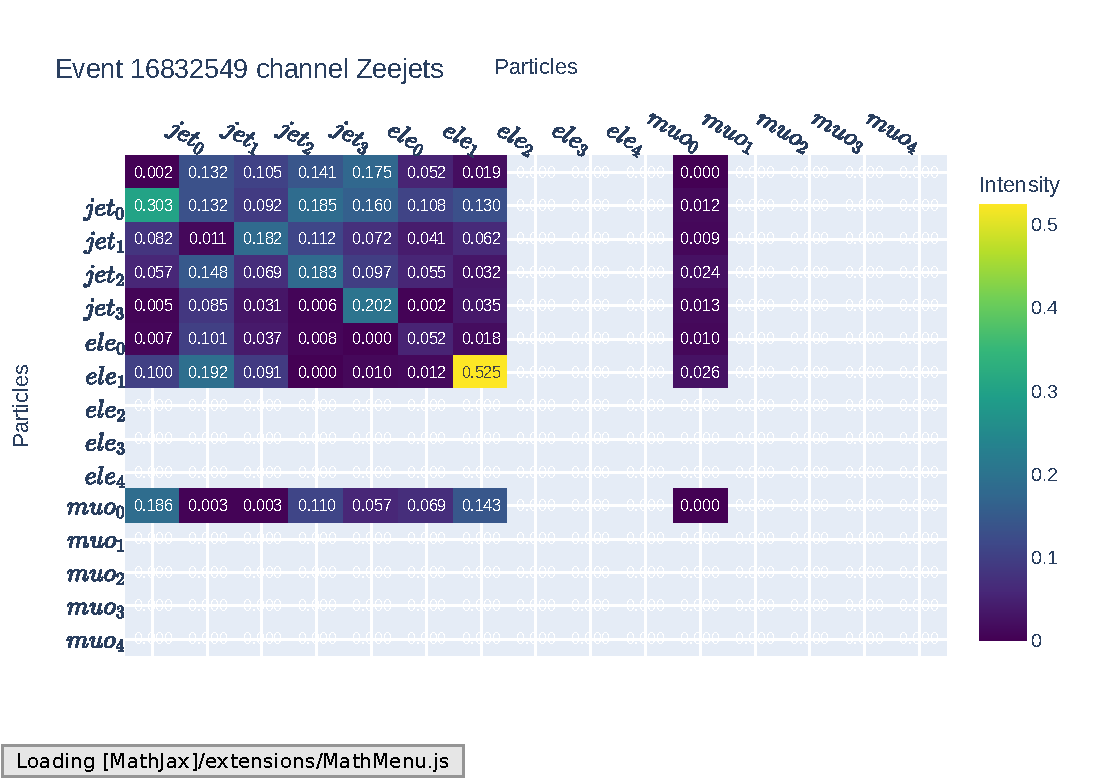
\includegraphics[width=\textwidth]{Figures/rmms/rmm_event_16832549_Zeejets.pdf}
        \caption{RMM matrix for event number 16832549 from the MonteCarlo Zeejets sample. Each feature is scaled based on a fit for that feature for all events in the training set ($\approx 80\%$ of total MC)}
        \label{fig:rmm_zee_event}
    \end{subfigure}
    \hfill
    \begin{subfigure}{.7\textwidth}
        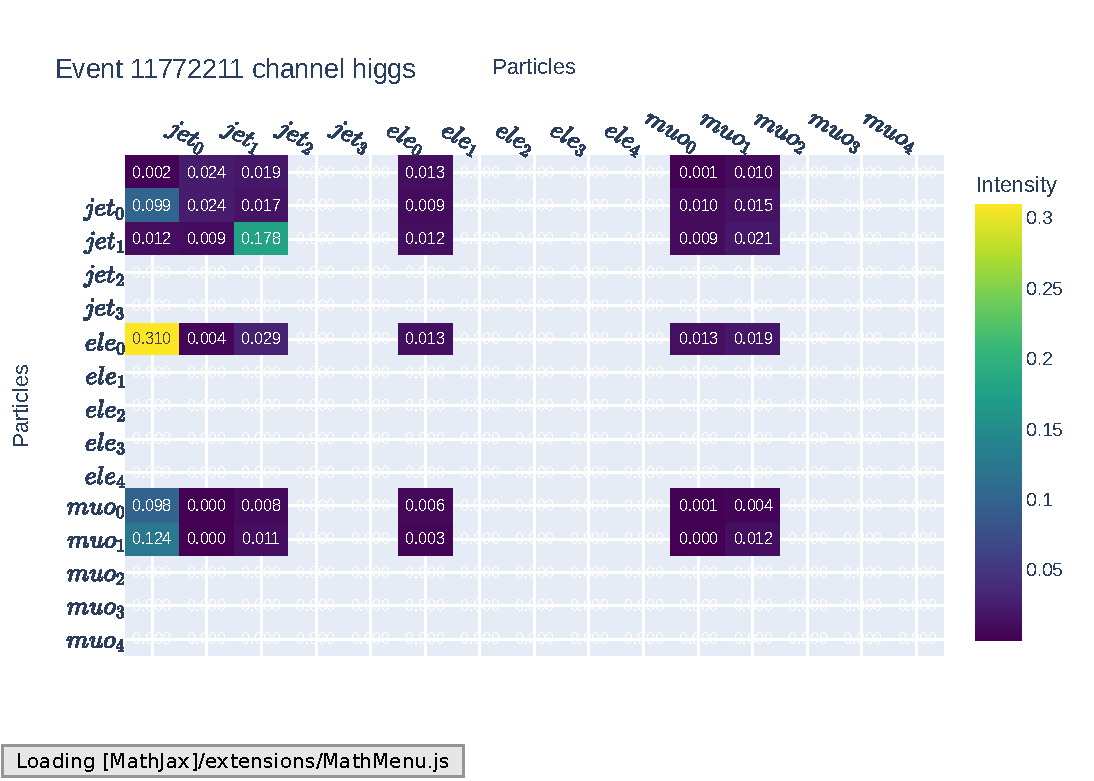
\includegraphics[width=\textwidth]{Figures/rmms/rmm_event_11772211_higgs.pdf}
        \caption{ RMM matrix for event number 11772211 from the MonteCarlo Higgs sample. Each feature is scaled based on a fit for that feature for all events in the training set ($\approx 80\%$ of total MC)}
        \label{fig:rmm_higgs_event}
    \end{subfigure}
    \hfill        
    \caption{}
    \label{fig:rmm_singular_events}
\end{figure}

In figure \ref{fig:rmm_singular_events} we see two RMM matrices created from two different channels in the MonteCarlo samples. This RMM is of type T3N5\footnote{T3 $\to$ 3 particle types: jets, electrons and muons. N5 $\to$ 5 particles per particle type. Note here that we have 5 particles only for the leptons, and 4 particles for the jets.}. 
These RMM matrices have scaled the features that a minimum value less than $-3$ and or a maximum value of above $3$. These scalers were fitted to the specific value using the "$.fit\_transform()$" and "$.transform()$" 
functions from the Scikit-learn library\cite{scikit-learn}. For easier interpretability, the gray area corresponds to a missing value, leading to so called "islands" in the RMM matrix.


\subsection*{MonteCarlo and data comparison}\label{sec:mcdatacomp}

Before we can start the analysis, we need to compare the MonteCarlo and data. This is done to ensure that the training samples we use are actually useful. As described by R. Stuart 
Geiger et al. \cite{DBLP:journals/corr/abs-2107-02278}, the concept of "Garbage in, garbage out" is of key importance in computer science, and indeed important in high energy physics. 
To ensure that the models we train actually learns physical processes, the training set must represent the physics "status quo". If the training samples do not match the physical reality,
we regard it, in the context of high energy physics, as garbage in, which will in turn give garbage out. The Monte Carlo standard model simulations are indeed very good, but the are 
numerical approximations, and can sometimes be off. Thus, every feature that well be used for training have to be checked before being used. This is done by comparing the distributions 
of the features in the MonteCarlo and ATLAS data. Assuming that there are no issues with the data collection from ATLAS, we then assume that the data from ATLAS is the "ground truth", as it 
is the only dataset we can analyze, and the only dataset we can compare to. The MonteCarlo is then compared to the data, and if the distributions are similar, we can assume that the 
training samples are good enough. 


\begin{figure}[h!]
    \centering
    \begin{subfigure}{.6\textwidth}
        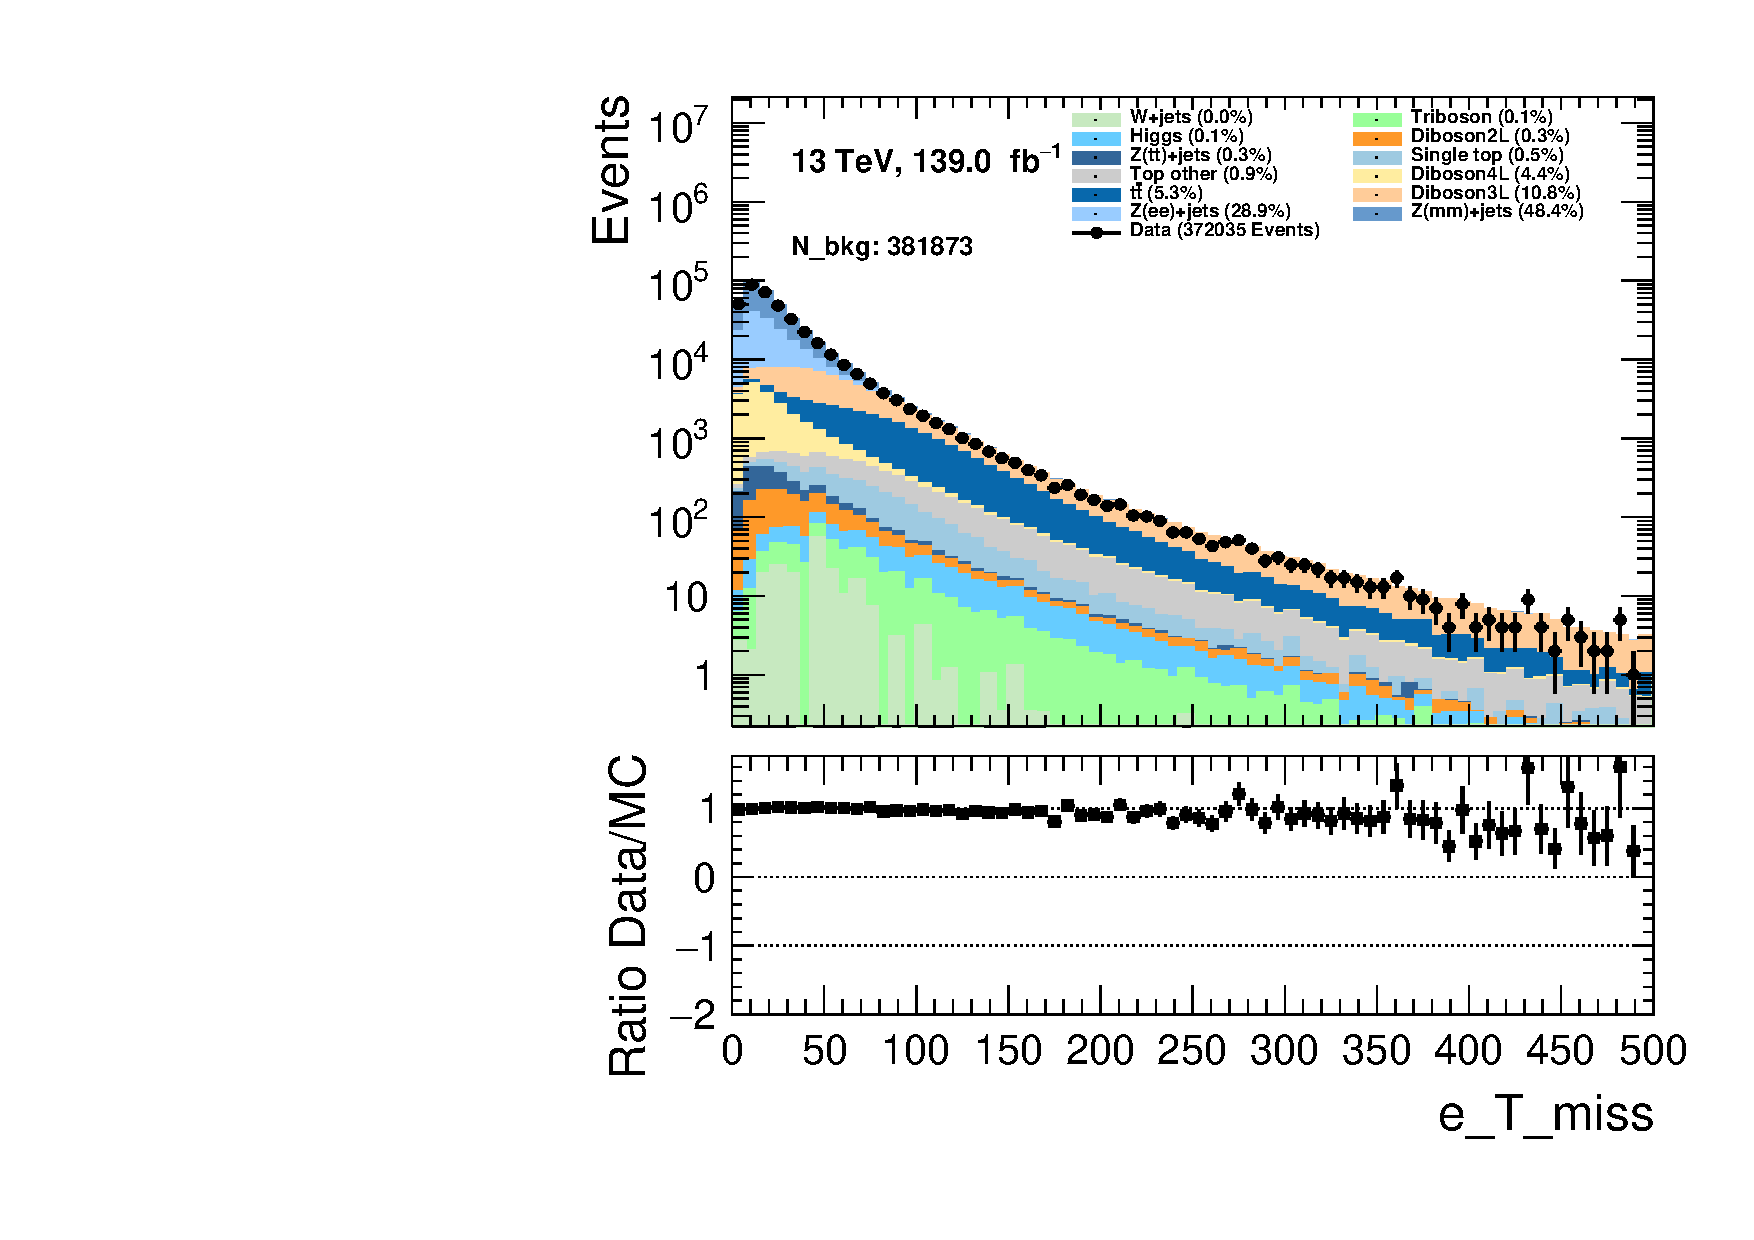
\includegraphics[width=\textwidth]{Figures/MC_Data_comp/e_T_miss.pdf}
        \caption{Missing transverse energy for the three lepton final state. The histogram contains the entire Run 2 dataset.}
        \label{fig:etmiss}
    \end{subfigure}
    \hfill
    \begin{subfigure}{.6\textwidth}
        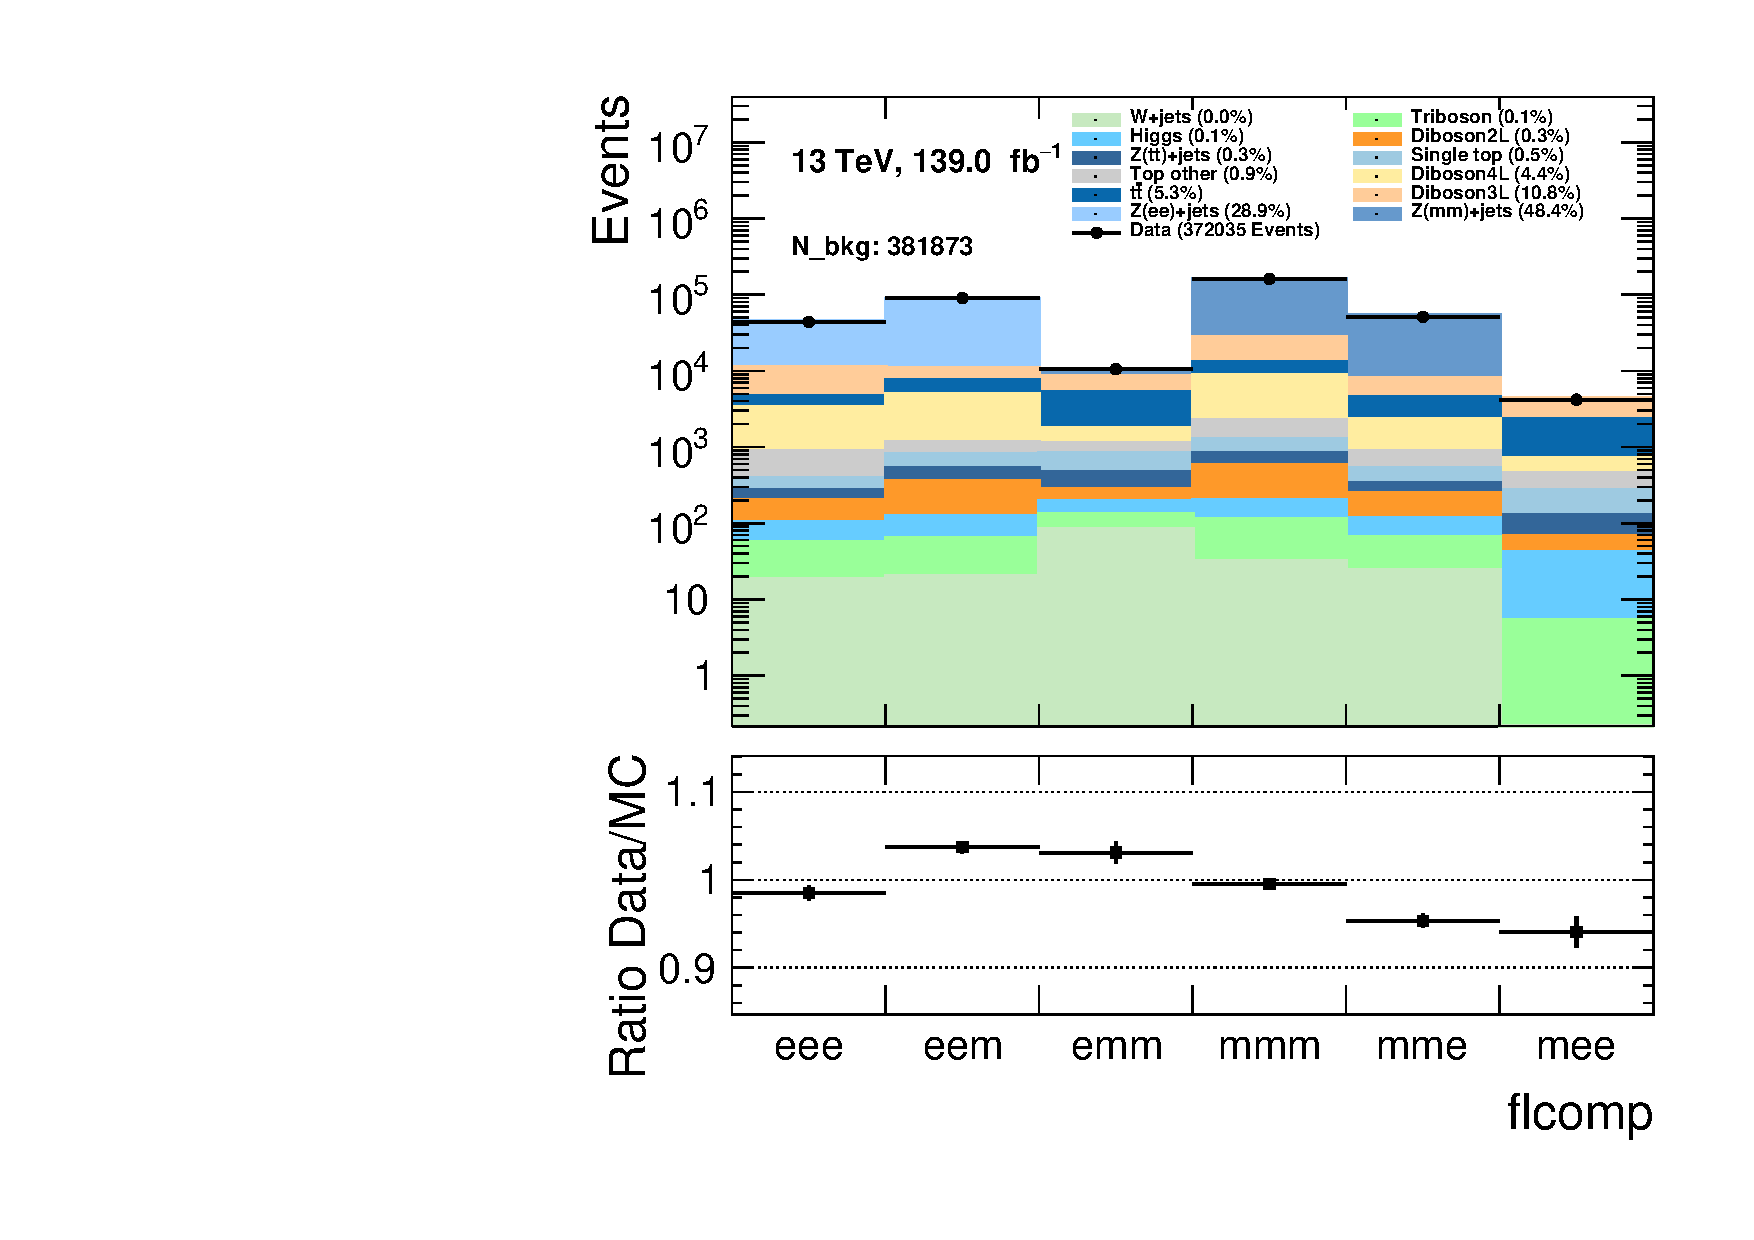
\includegraphics[width=\textwidth]{Figures/MC_Data_comp/flcomp.pdf}
        \caption{Flavor combination for the three lepton final state. This histogram only contains the flavor combinations for the good leptons, denoted $lep_{SG}$. The histogram contains the entire Run 2 dataset. }
        \label{fig:flcomp}
    \end{subfigure}
    \hfill        
    \caption{Comparison of the MonteCarlo and data for the three lepton final state with the features $e_{T}^{miss}$ and flavor composition.
    }
    \label{fig:MC_Data_comp}
\end{figure}

In figure \ref{fig:MC_Data_comp} two features have been selected to vizualize the comparison between Monte Carlo and ATLAS data, $e_T^{miss}$ and $flcomp$. 
We see that both $e_T^{miss}$ and $flcomp$ satisfy a good ratio between Monte Carlo and ATLAS data, thus we can safely move forward with the analysis. 
All features were checked, and can be found in appendix B.
\par \par

\subsection*{Tabular data}